\documentclass{beamer}

\usepackage{verbatim}
\usepackage{url}
\usepackage{xcolor} % See documentation PDF at http://www.ctan.org/pkg/xcolor
\definecolor{darkgreen}{rgb}{0,0.3,0}
\definecolor{lightgrey}{rgb}{0.65,0.65,0.65}
\usepackage{tikzsymbols}


\setbeamertemplate{section in toc}[sections numbered]
\setbeamertemplate{subsection in toc}[subsections numbered]
\setbeamertemplate{subsubsection in toc}[subsubsections numbered]
\usetheme{Singapore}
\setbeamertemplate{navigation symbols}{}
\setbeamertemplate{footline}{%
\vspace{0.0em}%
\hspace{0.5em}%
{\color[rgb]{.1,.1,.1} \insertframenumber{}~/~\inserttotalframenumber}
}

\newcommand{\code}[1]{{\color{darkgreen}\texttt{#1}}}
\newcommand{\detail}[1]{{\color{lightgrey}\small{}#1}}


\begin{document}

\title{Probabilities, probably \\[1.5em]
 %{\Huge ¯\\\_(ツ)\_/¯}
 %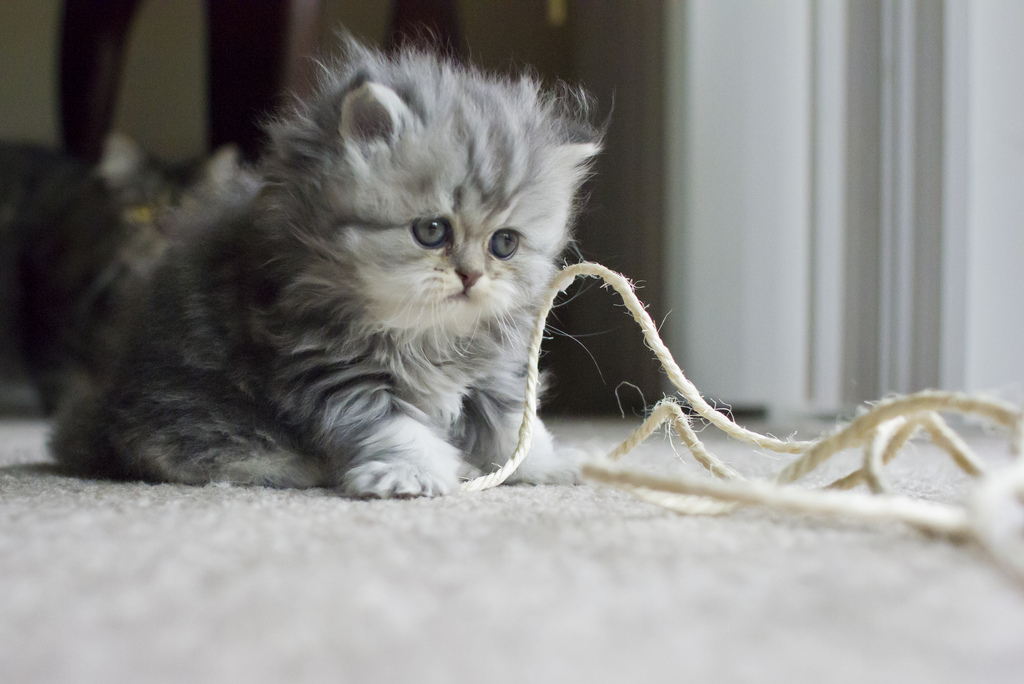
\includegraphics[width=0.5\textwidth]{images/kitten_string_flickr_albaraa.jpg} \\[-1.0em]
 %\small{Possibilities} \\[1.0em]
 %LT1 \\[1.0em]
 }
\author{\href{http://jon.dehdari.org}{Jon Dehdari}}
\frame{\titlepage}

\begin{frame}{Good Morning!}
	\begin{center}
		\only<1>{
\includegraphics[width=0.8\textwidth]{images/anything_is_possible.jpg}}
		\only<2>{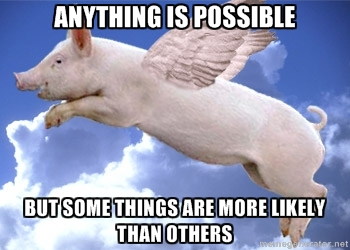
\includegraphics[width=0.8\textwidth]{images/flying_pig.jpg}}
	\end{center}
\end{frame}

\begin{frame}{Fifty Shades of Nay}
\begin{itemize}
	\item Last week we discussed (formal) languages and grammars in terms of \textbf{set membership}
	\pause
	\item That is, whether a particular sentence was \textbf{grammatical} or \textbf{ungrammatical}
	\pause
	\item This is, of course, an overly simplistic view of natural language
	\pause
	\item This week, we're going to take a more subtle approach
	\item The formal languages \& grammars are still relevant, but we're going to add \textbf{probabilities} to them
\end{itemize}
\end{frame}

\begin{frame}{Probability}
\begin{itemize}
	\item A \textbf{probability} tells you how likely something will happen
	\pause
	\item Another way of looking at it is that it is just a score for a possible event
	\pause
	\item The score is between 0 and 1 \detail{(the unit interval)}
	\item The scores for all of the possible outcomes must add up to 1 \detail{(unity)}
	\pause
	\item Adding up all the scores is called \textbf{normalization}
	\pause
	\item A \textbf{probability distribution} is the probabilities for all the possible outcomes
\end{itemize}
\end{frame}


\begin{frame}{Probs, cont'd}
\begin{itemize}
	\item A \textbf{uniform distribution} is where all the outcomes have the same probability
	\pause
	\item That's rarely true in the real world
	\pause
	\item But it's a good starting point, until you know better
	\pause
	\item So, for example, suppose I say ``It's raining cats and \underline{\hspace{2em}}'' .  \pause What word do you think I'll say next?
	\pause
	\item A uniform distribution would give the same probability for every English word
	\vspace*{-1.0em}
	\begin{footnotesize}
	\begin{eqnarray*}
	 p(w_i) & = & \frac{1}{|V|} \\
	        & = & |V|^{-1} \\
	\end{eqnarray*}
	\end{footnotesize}
	\vspace*{-2.0em}
	\pause
	\item Ok, so maybe it's not a very good idea
\end{itemize}
\end{frame}


\begin{frame}{Unigram Distribution}
\begin{itemize}
	\item In a \textbf{unigram distribution} (or unigram model), probabilities are based on word frequencies
	\pause
	\begin{eqnarray*}
	 p(w_i) & = & \frac{\text{count}(w_i)}{\text{count}(w)} \\
	\end{eqnarray*}
	\vspace*{-2.0em}
	\pause
	\item So the word ``the'' will have a much higher probability than ``dogs''
	\pause
	\item It doesn't take into account a word's context
\end{itemize}
\end{frame}


\begin{frame}{}
\begin{itemize}
	\item The probability of two events occurring is called the \textbf{joint probability} \ \detail{$p(h,w)$}
	\pause
	\item The probability of a \textbf{w}ord after a \textbf{h}istory of previous words is the \textbf{conditional probability} \ \detail{$p(w|h)$}
	\pause
	\item The reverse of that is the \textbf{posterior probability} \detail{$p(h|w)$}
	\pause
	\item The \textbf{prior probability} tells us how probable the word is, in its own right \ \detail{$p(w)$}
	\pause
	\item \textbf{Likelihood} is the probability of the entire data, given our model.  \pause The higher this is, the better it is at predicting the data...
\end{itemize}
\end{frame}

\begin{frame}{How good are you at guessing?}
\begin{itemize}
	\item Likelihood is usually a really really small number.  Why?
	\pause
	\item People often transform this really small number to a large negative number via the logarithm function \ \detail{(log$_2$)}
	\item This is then called the \textbf{log likelihood}
	\pause
	\item Not content there, ``people'' then remove the negative sign, making it a positive number
	\item Then they'll divide that number by the number of words in the data.  Why?
	\pause
	\item This gives us the average number of binary choices the model made to predict each outcome in the data, or \textbf{cross entropy}
\end{itemize}
\end{frame}


\begin{frame}{I'm Perplexed}
\begin{itemize}
	\item Cross entropy also tells us how different two distributions are, like the model and the data \ \detail{$H(\theta, {\bf x})$}
	\pause
	\item If we take the binary exponent of the cross entropy ($2^H$), we get \textbf{perplexity}
	\pause
	\item This is how confused the model is, on average
	\pause
	\item In other words, perplexity (PP or PPL) is the average number of words that the model guessed for each trial in the data
	\pause
	\begin{center}
		\vspace*{0.5em}
		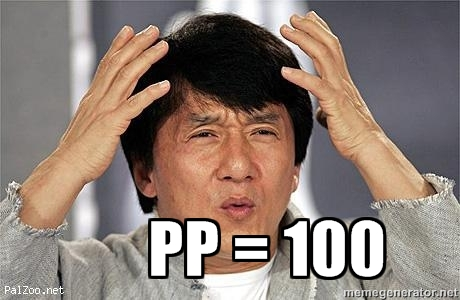
\includegraphics[width=0.3\textwidth]{images/jackie_chan_perplexity.jpg}
	 \end{center}
\end{itemize}
\end{frame}

\begin{frame}{Entropy}
\begin{itemize}
	\item \textbf{Entropy} measures how predictable the data is
	\pause
	\begin{equation*}
	H(X) = - \sum_{x \in X} p(x) \log_2 p(x)
	\end{equation*}
	\pause
	\begin{center}
		\vspace*{0.5em}
		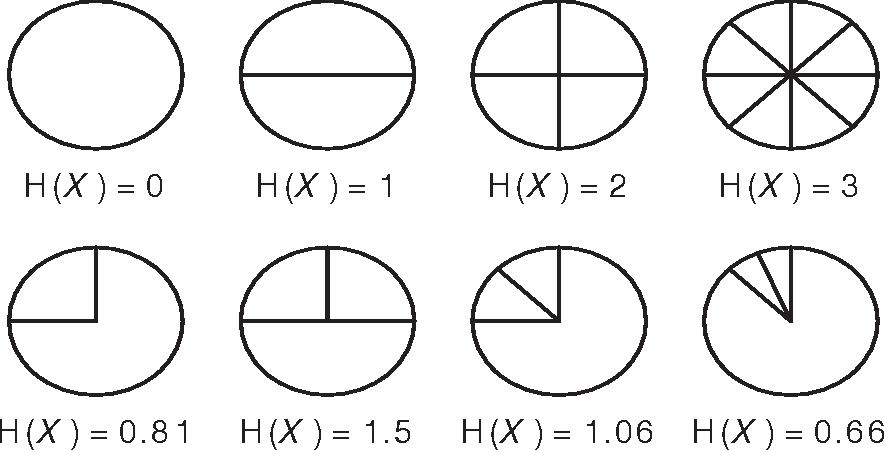
\includegraphics[width=0.7\textwidth]{images/koehn_2010_fig_3_4.pdf}
	 \end{center}
	{\tiny (courtesy of Koehn, 2010)}
\end{itemize}
\end{frame}


% sample, interpolation, entropy

\begin{frame}{Maximum Likelihood Estimation}
\begin{itemize}
	\item \textbf{Maximum likelihood estimation} (MLE) just uses counts/frequencies of seen events in the train data
	\item Why is this type of estimation called \textit{maximum likelihood}?
	\pause
	\item Are there ever any unseen events in language data?
	\pause
	\item How could we handle unseen events (not seen before in the training set)?
\end{itemize}
\end{frame}


\begin{frame}{Rule-based and Statistical NLP}
\begin{itemize}
	\item Rule-based models are a subset of statistics-based models
	\pause
	\item Rules have an unsmoothed, uniform distribution -- each rule has an equiprobable chance
	\pause
	\item Grammatical: $p(x) > 0$\,, ungrammatical: $p(x) = 0$
\end{itemize}
\end{frame}

% \begin{frame}{}
% \begin{itemize}
% 	\item 
% 	\item 
% 	\item 
% \end{itemize}
% \end{frame}


\end{document}
